% En esta sección se deben explicar los riesgos que se materializaron a lo largo del
% proyecto, estuvieran o no previstos al comienzo (más aún si no estaban previstos).
% Por ejemplo, desvíos en las estimaciones que hayan obligado a modificar el alcance,
% interesados con los que esperaban contar que finalmente no estuvieron disponibles, 
% metodologías o tecnologías que no funcionaron como se esperaba, y cuestiones de 
% este estilo.
% Los riesgos no previstos son per se lecciones aprendidas, pero también resulta de 
% interés explicitar qué aspectos del proyecto les dejaron lecciones positivas que 
% hayan servido para el aprendizaje.

\noindent A continuación detallamos los problemas encontrados a lo largo del desarrollo del
Trabajo Profesional, así como también las lecciones que aprendimos de ellos. Estos problemas fueron en su mayoría imprevistos que o bien
dificultaron el progreso o bien imposibilitaron el desarrollo de ciertas funcionalidades deseadas originalmente.

\subsection{Kubernetes}
\label{sec:lessons-kubernetes}

\noindent En la sección \ref{sec:kubernetes} explicamos que utilizamos Kubernetes como ambiente de despliegue productivo para
el servidor. La problemática de utilizar Kubernetes como entorno de despliegue es que no existen servicios gratuitos que lo ofrezcan,
lo más cercano que ofrecen algunos pocos proveedores Cloud es un período de prueba de típicamente 30 días combinado con un sistema de
créditos iniciales que se consumen al utilizar los servicios. Tal es el caso de Google Cloud, Digital Ocean y Microsoft Azure, al menos al momento
de la realización de este Trabajo Profesional.

Inicialmente intentamos desplegar la aplicación en GKE, el servicio de Kubernetes de Google, y valernos de los 30 días de prueba iniciales. Lamentablemente,
parece que la configuración de GKE no es compatible con Akka, dado que se generaban errores al momento en el que los nodos intentaban descubrirse entre sí vía
DNS. No logramos encontrar solución ni en los foros de Akka ni en los de GKE, y las opciones de configuración de red de Google resultaron ser insuficientes para
solucionar el problema.

Intentamos luego con Digital Ocean, pero el cluster de Kubernetes gratuito ofrecido resultó insuficiente para lograr ejecutar más de un nodo de la aplicación, por lo que
tuvimos que descartar esta opción también. Microsoft Azure resultó prometedor; logramos formar el cluster de Akka correctamente y la aplicación se comunicaba correctamente entre
los distintos nodos. Sin embargo, al momento de conectar a un jugador, el \textit{firewall} de Azure bloqueaba la conexión constantemente. Configuramos el firewall con las reglas necesarias
en principio, pero continuamos sin conseguir que acepte el tráfico del cliente.

Finalmente, como último intento de proveedor Cloud, utilizamos Amazon Web Services. AWS no ofrece créditos de regalos para EKS, su implementación de Kubernetes, sino que factura por tiempo
de uso de los recursos y tráfico externo de la red. Sorprendentemente, la misma configuración que no hicimos en los otros proveedores y dio distintos problemas en cada uno, funcionó correctamente
en AWS. La aplicación se desplegó correctamente y podíamos conectar clientes sin problemas. Por otro lado, debido a los altos costos de Amazon para su implementación de Kafka (MSK) optamos por utilizar
tanto servicios de \textit{hosting} gratuitos para Kafka como para PostreSQL, siendo \textbf{CloudKarafka} y \textbf{ElephantSQL} los servicios utilizados respectivamente.

Si bien el ambiente productivo Cloud nos fue de utilizada durante unas semanas, finalmente decidimos que debíamos ir a una solución que nos permitiera mantener el ambiente de producción funcionando constantemente
y ejecutar pruebas de carga sin incurrir en costos muy elevados ni vernos limitados por los servicios gratuitos de infraestructura. Además, tanto CloudKarafka como ElephantSQL anunciaron la baja de servicio
durante el 2024 (ambos son desarrollados por la misma empresa), por lo que todo nos llevó a desarrollar nuestro ambiente productivo actual.

Decidimos ir, finalmente, por una solución \textbf{\textit{self hosted}}. Construimos nuestro propio cluster de Kubernetes conformado por 3 nodos RaspberryPi. En particular nos decantamos por la distribución de
\textbf{k3s} de Kubernetes, por su facilidad de instalación y configuración, especialmente para RaspberryPi. El cluster es de tipo High Availability (HA), ya que cuenta con los 3 nodos como nodos servidor, es decir,
si un nodo falla el cluster puede seguir operando correctamente. Las RaspberryPi, al ser SBCs (Single Board Computers) de bajo consumo, nos permitieron mantener el ambiente productivo en funcionamiento
constante, mientras que antes debíamos levantar el ambiente únicamente para realizar pruebas debido a su alto costo de uso. Esto resultaba además en tiempo desperdiciado, ya que en EKS la única forma de evitar costos adicionales
cuando no estuviéramos utilizando el cluster era eliminarlo, por lo que debíamos esperar a su recreación cada vez que quisiéramos utilizarlo.

\begin{figure}[htbp]
    \centering
    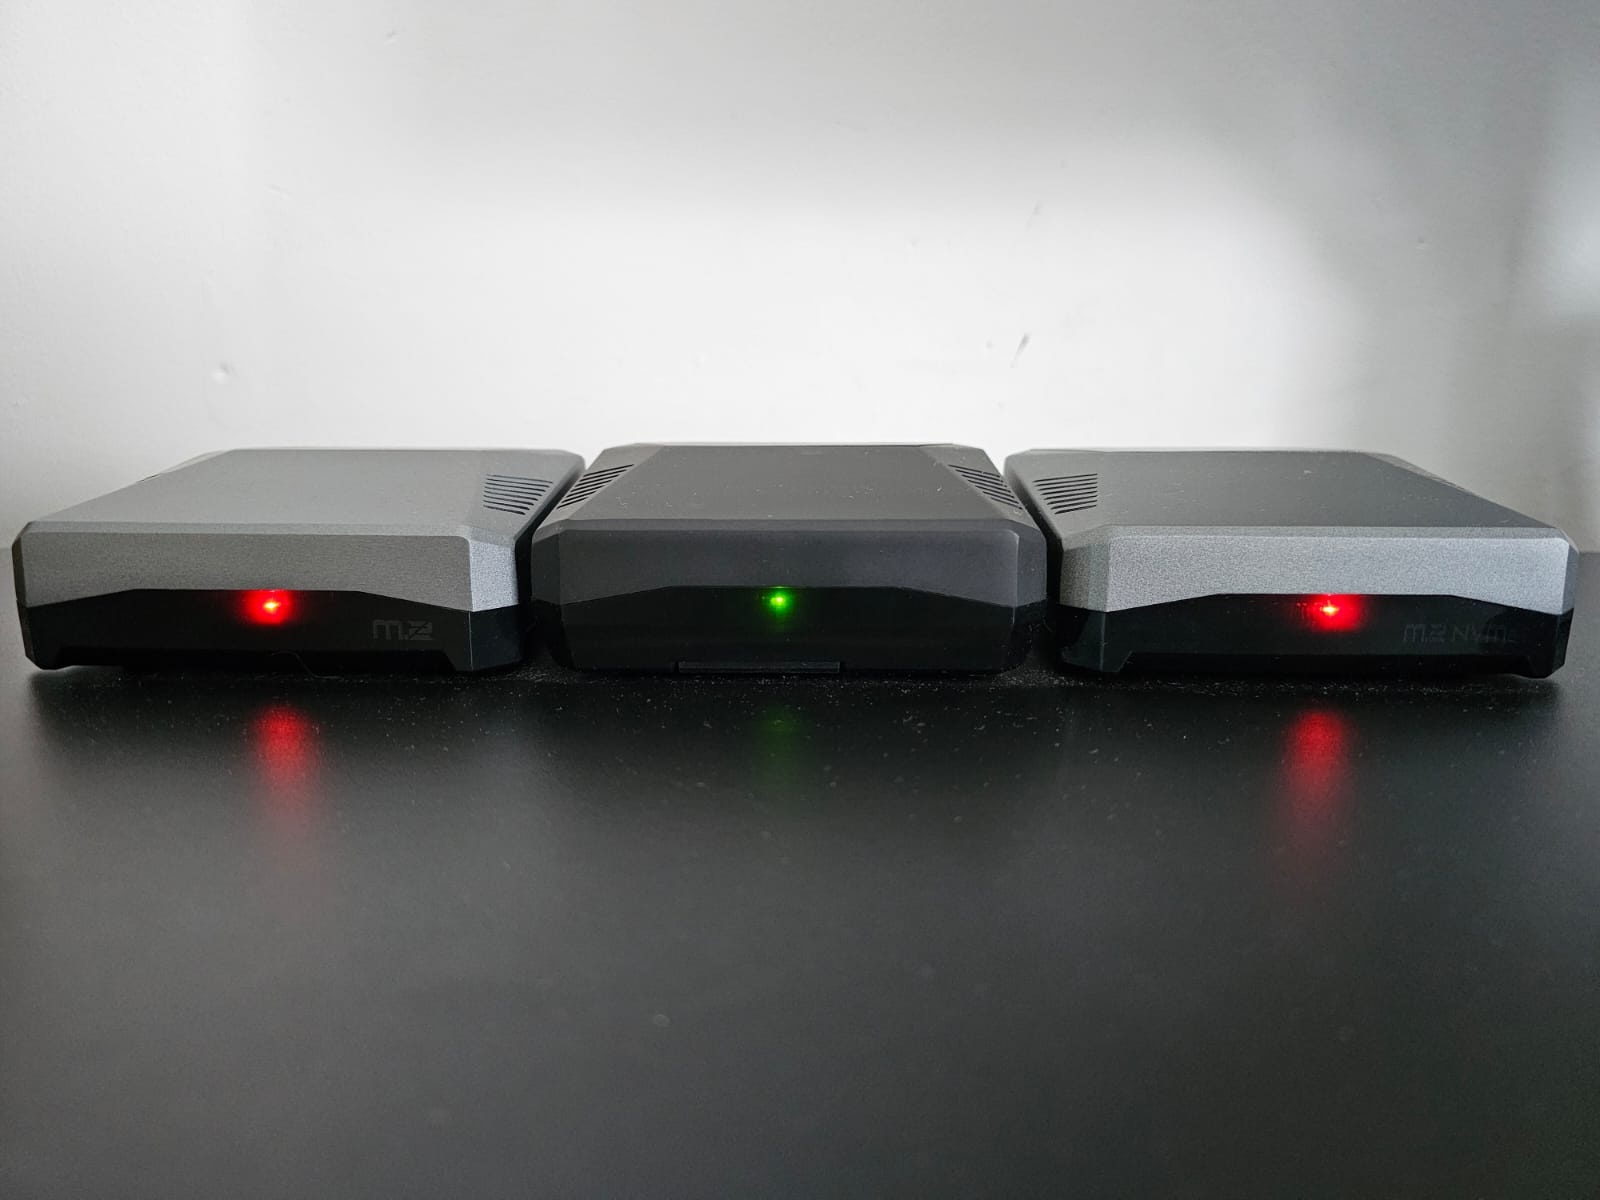
\includegraphics[width=0.8\textwidth]{../assets/fiubakka-cluster-pis.png}
    \caption{Cluster de Kubernetes utilizado en \textit{Fiubakka}.}
\end{figure}

Por otro lado, al utilizar un cluster propio en lugar de manejado por algún proveedor Cloud, surgió la problemática de como exponer los servicios a la red pública. Existen distintas formas de conseguir esto, desde la más cruda vía
exposición de ports (conocido como \textit{Port Forwarding}) hasta la utilización de servicios externos que ofrecen \textit{proxies} para mayor seguridad y abstracción. Nosotros optamos por esta segunda opción, haciendo uso de
\textbf{Cloudflare} \label{ref:cloudflare}. En particular, utilizamos \textbf{Cloudflare Tunnel} para exponer los distintos servicios a la red pública. Cloudflare lo ofrece de manera gratuita, lo único que tuvimos que pagar fue el dominio (vía Cloudflare
también) que utilizamos para exponer los servicios. El servidor de \textit{Fiubakka} se encuentra expuesto a través de \textbf{fiubakka.marcosrolando.uk} en el puerto 2020, y lo que se expone es un balanceador de carga TCP de Kubernetes
para poder distribuir las conexiones entre los distintos nodos del servidor.

\subsection{Funcionalidades descartadas}

Si bien se lograron implementar tanto la arquitectura del Servidor distribuido que es el objeto
de estudio de este Trabajo así como también el juego que funciona como interfaz de aplicación
para los usuarios, existen algunas funcionalidades para el juego que fueron inicialmente
planeados pero por restricciones de tiempo no fue posible completarlos. A continuación, listamos 
las mas interesantes:

\subsubsection{Sistema de recompensas y tienda de ítems}

\noindent Así como existen muchos cosméticos para la creación del personaje y además es posible cambiarlos dentro del
juego, no existe para los jugadores alguna forma de obtener nuevos cosméticos además de los que poseen en sus
inventarios. Para solucionar esto, surgió la idea de agregar un tipo de moneda con la cuál un usuario podría comprar nuevos
items equipables. Dichos objetos podrían ser adquiridos en una tienda ubicada en el \textbf{Level} del \textbf{Comedor}.

Esta funcionalidad hubiese estado relacionada al \textbf{Truco}, ya que la adquisición de esta moneda
sería una recompensa por ganar partidas de \textbf{Truco}.

\subsubsection{Foro de consultas}

\noindent Teniendo en mente la temática de una facultad, donde uno suele juntarse con profesores y/o compañeros de clase
para intercambiar ideas o hacer consultas, también se pensó en implementar un foro de consultas donde un usuario
podría realizar un \textit{post} a modo de consulta y los demás usuarios podrían responder a la misma. Tanto el \textit{post}
original como las respuestas podrían recibir votos positivos o negativos de parte de cualquier usuario, con el fin
de poder votar la "mejor respuesta". Esta funcionalidad se inspira en foros y páginas de consulta como lo es por ejemplo
\textit{StackOverflow}.

Para realizar una consulta dentro del juego, un jugador podría hacerla acercandose a una pizarra y creando el \textit{post}.
Si bien el chat es una forma de comunicación por texto entre jugadores, carece de la persistencia necesaria que necesitaría
una consulta que puede ser respondida luego de mucho tiempo, ya que el log de mensajes del chat se borra cuando el jugador
cierra el juego.

\subsubsection{Clases de programación}

\noindent Una idea que surgió naturalmente dada la ambientación del juego fue la de tener minijuegos relacionados a distintas materias
de la facultad. De todos los minijuegos que se nos ocurrieron, el más interesante era sin dudas el que apuntaba a simular
una clase de programación. El jugador ingresaría a una sala similar a los laboratorios del piso 4 y al interactuar con una
computadora, vería una interfaz como si fuera un \textit{IDE}. Allí tendría una consigna y la posibilidad de escribir código.
Una vez finalizado, ese código se analizaría para ver si resolvía correctamente la consigna y en ese caso, podría pasar a una nueva
consigna mas compleja.
% TODO: Como íbamos a mandar el codigo? Me suena que era con Kafka, pero nose si ya habiamos encontrado una herramienta
% para analizar el codigo submiteado

\subsection{Godot Editor}

\subsubsection{Godot: Optimización de imágenes}

\noindent En cierto punto del desarrollo, nos encontramos con que cargar el proyecto en el editor de Godot
requería alrededor de 3 GB de memoria RAM y levantar una sola instancia del juego requería además
otros 3 GB extra en memoria principal. En un entorno de desarrollo donde es necesario testear
funcionalidades teniendo por lo menos dos instancias del juego corriendo a la vez, esto dificultó e incluso
imposibilitó para algunos integrantes continuar normalmente con el desarrollo. Este requerimiento
de RAM no parecía tener sentido, ya que la suma del espacio requerido en disco de todos los 
\textit{assets} de nuestro proyecto no superaba los 100 MB.

Luego de investigar más a fondo el problema y entender cómo estábamos cargando los archivos de imágenes,
entendimos mejor el mecanismo que usa Godot para importar imágenes y qué implica eso.

Al agregar una imagen al proyecto, Godot genera automáticamente un archivo con el mismo nombre y extensión
\textit{.import}, con metadata y configuraciones del archivo. 
Por ejemplo, para el caso de las imágenes, es posible configurar el modo de compresión, generación de 
\textit{mipmaps}, entre otras opciones. Godot un modo de compresión \textbf{Lossless} por defecto. 
Si bien este modo tiene la ventaja de que no genera artefactos visuales en las imágenes importadas, usa 
considerablemente más memoria VRAM (\textit{Video Random Access Memory}) para almacenar la textura o
imagen importada, en comparación con otras opciones de compresión disponible.
La documentación de Godot\cite{ref2} provee un estimado del espacio que ocupa una sola textura
RGBA8 en la VRAM, dependiendo de las dimensiones de resolución de la imagen y del método de compresión utilizado.
En nuestro caso, como tenemos una imagen \textit{spritesheet} por cada variante de cada cosmético posible para los jugadores,
contábamos con más de 100 imágenes de más de 2048 x 2048 pixeles cada una. 

\begin{figure}[htbp]
    \centering
    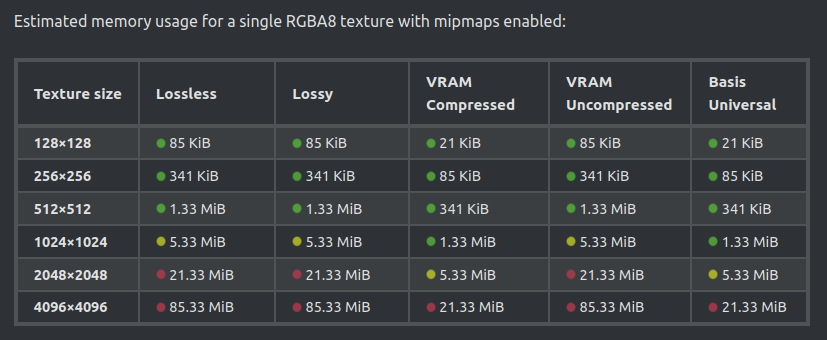
\includegraphics[width=1.0\textwidth]{../assets/godot-docs-images.png}
    \caption{Cuadro comparativo del tamaño que ocupa una imagen en VRAM según la resolución
             de la misma y el modo de compresión utilizado.}
\end{figure}

Usando de referencia la tabla de la documentación, y considerando que nuestras imágenes superaban
los 2048 x 2048 pixeles, además de estar usando el método de compresión Lossless,
la memoria en VRAM requerida para nuestro juego alcanzó una cota mínima de \textbf{2.24 GB}:

\[
\frac{21.33 \, MiB}{imagen} \times 100 \, imagenes = 2.24 \, GB
\]

Para computadoras sin una placa de gráficos dedicada, en lugar de alocar este espacio en VRAM,
se reserva en memoria principal RAM, generando los problemas anteriormente mencionados.
Habiendo entendido la causa de la problemática, aplicamos 2 soluciones para solventarla:

\begin{itemize}
    \item Reducir el tamaño de las imágenes recortándolas, ya que en realidad usamos solo
    una porción de la \textit{spritesheet}.
    \item Cambiar el modo de compresión de los cosméticos para personajes de \textbf{Lossless}
    a \textbf{VRAM Compressed}, para reducir aún más el espacio ocupado de VRAM. Si bien este
    modo de compresión no es recomendado para texturas 2D, especialmente del estilo
    \textit{pixel art} como lo es nuestro juego, al correr el juego usando este método de compresión
    no se notaron defectos ni artefactos visuales.
\end{itemize}

Tras haber implementado estos cambios, logramos reducir la memoria requerida por una instancia
del juego a menos de 1 GB.

\subsubsection{Control de versiones}

\noindent Uno de esos problemas está relacionado al control de versiones. Cada escena o nodo creado posee 
un archivo autogenerado por Godot en el cual se ven reflejados los cambios que realizamos desde 
el motor de videojuegos. No es usual que este archivo sea modificado manualmente, sino que toda 
modificación se realiza a través de la interfaz de Godot. Al realizar un merge con Github, si 
varias personas modificaron una misma escena o nodo, podría ocurrir que hubieran conflictos en 
dichos archivos autogenerados y al modificarlos manualmente, se eliminaran o modificaran líneas 
que terminaban ocasionando comportamientos no deseados en el juego.

Por ejemplo, para satisfacer los conflictos de un archivo podría haberse eliminado una signal 
que activaba alguna funcionalidad al presionarse un botón, y al no considerar que este botón 
podría dejar de funcionar al realizar el \textit{merge} de Github, este error era descubierto una 
vez que deseáramos presionar el botón. Debido a que el error fue introducido en un merge y 
no momentos antes de presionar dicho botón, la búsqueda del error podía tornarse complicada 
o confusa. Para prevenir estos problemas, observamos con más detenimiento los archivos 
autogenerados al momento de realizar merges y al momento de realizar code reviews, 
incluso dejando comentarios en los pull request preguntando si realizar dichos cambios 
es el comportamiento que el dueño del pull request está buscando.

\subsubsection{Uso de \textit{signals}}

\noindent Otro problema fue el acoplamiento de las escenas y los nodos. Durante gran parte del proyecto, 
la mayoría de los nodos se comunicaban con sus nodos hijos de la siguiente manera:

\begin{lstlisting}
    $nodo.metodo()
\end{lstlisting}

En un inicio, esta forma parecía resultar cómoda para poder llamar a los métodos de los nodos 
hijos, pero poseía un problema y era que el código se volvía difícil de reutilizar y refactorizar. 
Al utilizar signals en lugar de llamar a los métodos de los hijos de esta forma, no es necesario 
que el nodo padre y los nodos hijos conozcan detalles de la implementación del otro, aumenta 
la modularización, se puede intercambiar a los hijos de un nodo sin necesidad de modificar el 
código del padre, mejora la escalabilidad, por mencionar algunas ventajas.

\subsubsection{Convención en el nombramiento de \textit{callbacks}}

\noindent Relacionado al uso de señales, otro de los problemas que surgió es no seguir la convención de 
Godot al nombrar los callbacks creados manualmente para conectar a las señales:

\begin{lstlisting}
    _on_<nombre_del_nodo>_<nombre_de_la_signal>()
\end{lstlisting}

Al no saber qué nodo va a responder a una señal emitida, utilizar esta convención hace más 
fácil la búsqueda en el código.
